\section{Training Model} \label{sec:build3} Machine Learning models have previously worked wonders on the correct recognition of various algorithms when features extracted are fed into the model for it to figure out the false and the true cases. 

\begin{figure}[t]
	\DeclareGraphicsExtensions{.pdf,.png,.jpg}
	\begin{center}
		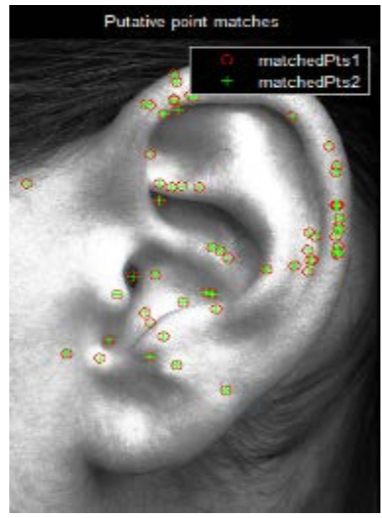
\includegraphics[width=0.5\textwidth]{Figures/Figure15}
	\end{center}
	\caption{The matching results of SURF detector}
	\label{fig:Figure15}
\end{figure}

\begin{figure}[t]
	\DeclareGraphicsExtensions{.pdf,.png,.jpg}
	\begin{center}
		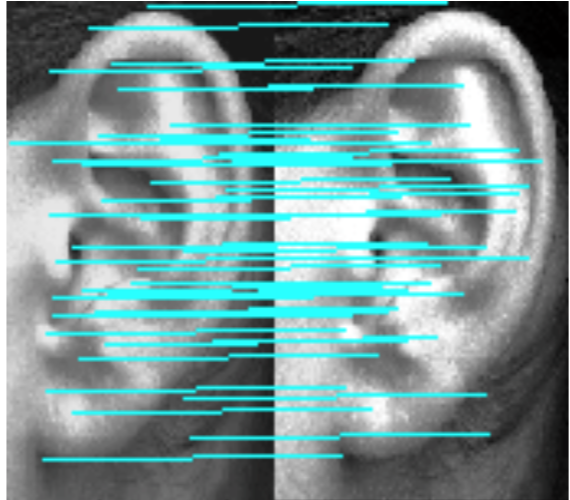
\includegraphics[width=0.5\textwidth]{Figures/Figure16}
	\end{center}
	\caption{The matching results of SIFT detector}
	\label{fig:Figure16}
\end{figure}


\begin{figure}[b]
	\DeclareGraphicsExtensions{.pdf,.png,.jpg}
	\begin{center}
		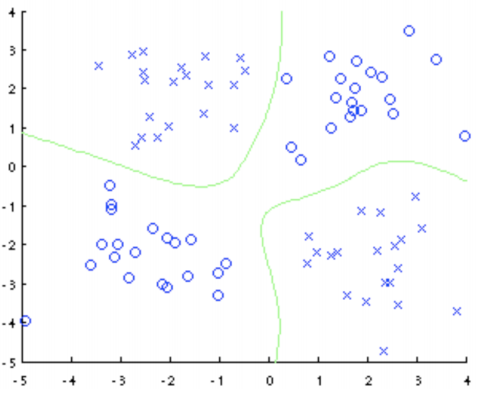
\includegraphics[width=0.5\textwidth]{Figures/Figure10}
	\end{center}
	\caption{Multi-class SVM(from \cite{libsvm})}
	\label{fig:Figure10}
\end{figure}

Support Vector Machines(SVMs)\cite{vapnik} brought a completely new idea to the field of machine learning. SVMs were introduced in COLT-92 by Boser,Guyon and Vapnik. For Pattern Recognition, SVMs have been used for Handwriting Recognition, Object Recognition, speaker identification, charmed quark detection, text categorization, face detection in images and many other purposes. SVMs are supervised learning models, with learning algorithms which are associated with it which are used to analyze data for classification and regression purposes. Given a set of training examples, each marked for belonging to one of two categories, an SVM training algorithm builds a model that assigns new examples into one category or the other, making it a non-probabilistic binary linear classifier. An SVM model is a representation of the examples as points in space, mapped so that the examples of the separate categories are divided by a clear gap that is as wide as possible. New examples are then mapped into that same space and predicted to belong to a category based on which side of the gap they fall on.

In addition to performing linear classification, SVMs can efficiently perform a non-linear classification using what is called the kernel trick, implicitly mapping their inputs into high-dimensional feature spaces.When data are not labeled, a supervised learning is not possible, and an unsupervised learning is required, that would find natural clustering of the data to groups, and map new data to these formed groups. The clustering algorithm which provides an improvement to the support vector machines is called support vector clustering and is often used in industrial applications either when data is not labeled or when only some data is labeled as a preprocessing for a classification pass.

SVMs can be divided into linear SVM and multi-class SVM, here we are more concerned with mulit-class SVM\cite{multiSVM}.

For our purpose we have used Multi-class SVMs. Support Vector Machines were originally designed for binary classification. The formulation to solve Multi-class SVM must have variables which are proportional to the number of different classes. The concept of SVM was proposed by Vapnik  et al. They helped to classify almost everything right from linear problems to multi-dimensional problems where the kernel matrix is use to transform the conflicting points into a different dimensional space called the kernel space in order to draw a hyperplane in a conclusive manner so as to separate the different cases. Here multiclass SVM is being used in order to classify the features as extracted by the various feature extraction techniques like SURF and SIFT. After that the model is trained and the features are matched with the features obtained from the query ear image in order to find a nearest match to succeed. Since it is multi-class, thus it helps to create separate classes for different classes of images and helps to classify them when the matching process is being done. The main process of better classification of the model depends on the input features. So as a matter of fact we can say that better the feature extraction is being done, better will be the classification made by the multiclass SVM and thus better will be the results.



